\section{Специфика предметной области}

С момента появления записывающей техники в области высокоэнергетических
экспериментов широкое распространение получила концепция эксперимента с
триггером~\cite{nucl-exp-methods-Grigorev1988}. В её рамках часть
детекторов выделяется в качестве триггерных,
а их сигналы обрабатываются логической функцией для принятия решения о записи
данных на основе откликов быстрых детекторов. Наличие или отсутствие сигналов
от определённого набора детекторов (составляющего лишь часть всего набора
детекторов установки и называемых \emph{триггерными детекторами}),
а также быстрая оценка физических величин
относительно заданных порогов, составляют входные параметры логического
условия. Срабатывание триггера задаёт временную точку отсчёта для
оцифровывания сигналов детекторов в некотором временном окне.
Совокупность данных записанных таким образом упорядочивается в рамках
структуры данных отдельного события. Классическим примером является
эксперимент Коуэна и Рейнеса по регистрации антинейтрино в
1954 году~\cite{cowan1956detection},
в котором основой для выделения событий взаимодействия антинейтрино с
протонами являлось фиксированная временная разница между чувствительными
элементами установки определяемая замедлением нейтронов в веществе
мишени.

Следует отметить, что понимаемый под (оцифрованным) \emph{событием}
набор данных в терминологии информационных систем не всегда строго
соответствует событию в вероятностном смысле. Хотя предполагается,
что события независимы, с определённой частотой — зависящей от
интенсивности исследуемого процесса — возможно наложение статистически
независимых событий во временных интервалах, определяемых длительностью
временного окна и инерционностью откликов детекторов. Этот эффект
естественно обусловлен физическими ограничениями, такими как время развития
электромагнитных и адронных ливней, лавинных процессов, а также
остаточной ионизацией в рабочих объёмах детекторов, сигналами от
вторичных частиц, гало пучка и т.д.

\subsection{Логический триггер}

В экспериментах с большим числом наблюдаемых каналов используется
многоуровневая триггерная система~\cite{nucl-exp-methods-Grigorev1988},
включающая триггеры различных
уровней (например, \emph{L1} — <<\emph{Level 1}>>, \emph{L2} и
последующие). Низкоуровневые аппаратные триггеры реализуются с
использованием аналоговых и дифференциальных схем, а также электроники
с наносекундным и пикосекундным временным разрешением. Их основная
задача --- обеспечить быстрый, предварительный отбор событий по сигналам
детекторов, подавляя таким образом комбинаторный фон сигналов от реакций,
не представляющих физического интереса.

Триггеры более высоких уровней, как правило, реализуются на менее
быстродействующей, но более гибкой цифровой компонетной базе:
на программируемых
логических интегральных схемах (\acrshort{fpga}), а также в виде
программных триггеров, выполняемых на
универсальных процессорах.

%То как именно соотносится программное представление события
%и его программная модель (цифровой образ) --- очень важный вопрос
%архитектуры \acrshort{sw} физического эксперимента.

Особое значение имеет то, каким образом соотносится информация о
событии и его цифровая модель в смысле логического соответствия
статически-типизированным данным. Этот аспект представляет собой ключевой вопрос
архитектуры программного обеспечения физического эксперимента, и его решение
можно можно сформулировать в виде различного рода формальных схем или
диаграмм.

%К примеру, проблема временного перекрытия событий, обусловленного
% чисто статистическими эффектами (для постоянной средней интенсивности
% временные интервалы между событиями подчиняются экспоненциальному распределению).
% В простейшем случае \acrshort{sw} может быть спроектировано таким образом, чтобы после записи событий
% от L1-триггера, события идентифицированные как pile-up отбраковывались и не учитывались в анализе. Такой подход
% не требует разрешать вклады от отдельных статистически-независимых событий. В тех случаях, когда
% интенсивность исследуемой реакции достаточно велика,
% чтобы результат измерений удовлетворял заданному порогу
% статистической значимости, а аппаратура подвержена влиянию
% сложных эффектов приводящих к трудноразрешимым
% неоднозначностям, такой подход оправдан и приводит к
% сравнительно простой архитектуре \acrshort{sw}:
% <<одна сигнатура --- одно событие>>.
% Более сложные случаи подразумевают присутствие в отклике детекторов информации о нескольких событиях, в том числе не обязательно сигнальных. В этом случае программная модель события уже не обязательно соответствует единственному исследуемому событию, хотя для упрощения задач анализа может быть целесообразно сохранить их логическую связь в виде выделенного программного представления.

К примеру, одной из характерных проблем в регистрационных системах является
временное перекрытие событий, обусловленное чисто статистическим
эффектом~(частотной перегрузке, перекрытием
сигналов, англ. \emph{pile-up}): при постоянной средней интенсивности временные
интервалы между событиями подчиняются экспоненциальному
распределению. На практике это означает, что в пределах одного
временного окна могут присутствовать отклики
от нескольких независимых событий.

В простейшем случае программное обеспечение может быть организовано
таким образом, чтобы после записи события, фильтрация, выполняемая при
анализе, отбраковывала записи, идентифицированные как результат
наложения событий, исключая их из дальнейшего анализа.
Такой подход не требует разрешения вклада от индивидуальных
статистически независимых событий и, при определённых условиях, оказывается
вполне обоснованным:
\begin{itemize}
    \item Если интенсивность исследуемого процесса достаточно высока для
    достижения необходимой статистической значимости результатов.
    \item Или если влияние аппаратурных эффектов приводит к возникновению
    неоднозначностей в интерпретации сигналов, которые затруднительно, или
    невозможно устранить алгоритмически.
\end{itemize}

В подобных случаях достигается относительная простота архитектуры \acrshort{sw},
основанной на принципе: <<одна сигнатура — одно событие>>.
В этом случае отношение между оцифрованным сигналом от детектора и
экземпляром события выглядит как простая ассоциация, изображённая на
рисунке~\ref{fig:simple-hit-event}, в котором тип данных~\texttt{Hit}
содержит информацию об отдельных откликах детектора, и его экземпляры
включены посредством композиции в экземпляр события представленный
типом данных~\texttt{Event} выражающим информацию об отдельном событии.

\begin{figure}[ht!]
    \centering
    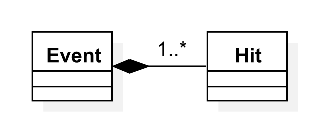
\includegraphics[width=0.25\linewidth]{images/illustrative/simple-event-struct.eps}
    \caption{Простейшая модель отклика детектора в событии}
    \label{fig:simple-hit-event}
\end{figure}

Более сложные сценарии предполагают, что отклик детекторной системы
может содержать информацию от нескольких перекрывающихся событий, включая
как сигнальные, так и обусловленные фоном. В таких условиях программная
модель записанного события инициированного триггерной системой уже не
обязательно соответствует одному акту взаимодействия.
Для упрощения дальнейшего анализа целесообразно
сохранять логическую связность таких данных в виде единого программного
представления (записи) о записи события по триггеру, при этом разделяя вклады
от различных первичных взаимодействий. Вариант реализации приведён на
рисунке~\ref{fig:complex-hit-event}, на котором тип данных события~\texttt{Event}
включает через композицию экземпляры типов данных с информацией об отдельных
откликах, объединяемых посредством агрегации в типе~\texttt{TimeCluster}.
Последний можно представить и в виде класса ассоциации в тех случаях, когда
по каким-то причинам необходима нормализация коллекции~(например, хранение в реляционной~\acrshort{db}).

\begin{figure}[ht!]
    \centering
    %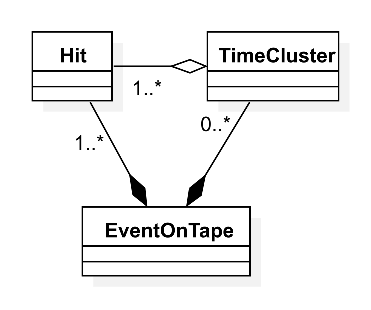
\includegraphics[width=0.33\linewidth]{imgs.view/illustrative/complex-event.eps}
    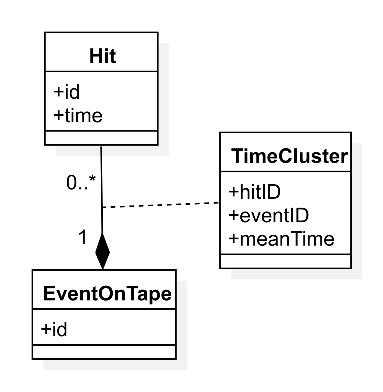
\includegraphics[width=0.33\linewidth]{images/illustrative/hit-assoc.eps}
    \caption{Модель события с разделением откликов во времени с классом ассоциации}
    \label{fig:complex-hit-event}
\end{figure}

В тех случаях, когда разделение откликов во времени неоднозначно, и конкурентные
гипотезы должны рассматриваться одновременно, может потребоваться введение
дополнительных классов ассоциации. На рисунке~\ref{fig:more-complex-hit-event}
вводится дополнительный тип данных~\texttt{Event} агрегирующий информацию о
конкурирующих гипотезах, выраженных посредством различной группировки
временных кластеров.

\begin{figure}[ht!]
    \centering
    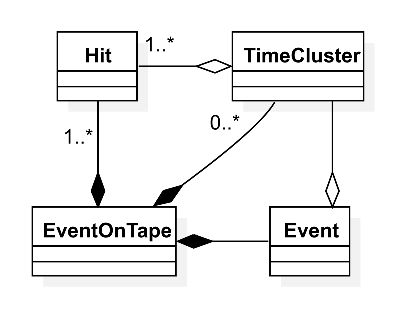
\includegraphics[width=0.33\linewidth]{images/illustrative/more-complex-event.eps}
    \caption{Модель события с разделением откликов во времени представляющая конкурирующие гипотезы}
    \label{fig:more-complex-hit-event}
\end{figure}

Описанные варианты организации модели события и его частей часто встречаются в
иерархии данных при обработке данных физического эксперимента. Другими примерами
могут быть треки частиц, образованные различными комбинациями пространственных
показаний трековых детекторов, амплитуды ячеистых калориметров образующие
пространственные кластеры, сигналы от многослойных трековых детекторов и т.д.
Различные способы представления составных типов данных включают кортежи,
таблицы, реляционных таблицы, структуры и классы, соответствующие выбранным
языковым средам.

\subsection{Модель события}

Среди доступных способов описать модель события в компьютерной программе выделим
следующие, как нашедшие наиболее широкое применение в практике организации
научного \acrshort{sw}:

\begin{itemize}
    \item \emph{Табличная модель}
    %описывает результаты
    %измерения отдельного события в виде кортежа~(строки)
    %%вещественных чисел~$v_i \in \mathbb{R}$
    %в котором
    %информация о принадлежности измерения $v_i$ кодируется
    %индексом~(колонкой)~$i$.
    представляет результаты измерений, относящихся к отдельному физическому событию, в виде
    кортежа (строки), компоненты которого интерпретируются как числовые значения,
    соответствующие различным характеристикам события. Идентификация каждого значения
    $v_i$ осуществляется посредством его позиции или имени соответствующего
    столбца $i$, что позволяет явно связать измеряемую величину с её смысловым
    назначением.
    \item \emph{Реляционная модель}
    %описывает событие в
    %виде наборов строк из взаимосвязанных таблиц между
    %которыми определены реляционные отношения. Для
    %эффективного использования этого подхода необходимо
    %соответствие модели т.н. \emph{нормальным формам},
    %описанным в теории реляционных таблиц.
    описывает событие как совокупность записей, организованных
    в виде взаимосвязанных таблиц, между которыми заданы формальные
    реляционные зависимости. Эффективное применение данного подхода требует
    приведения представления модели к формам,
    обеспечивающим согласованность и непротиворечивость представления,
    что формализуется в рамках т.н. \emph{нормальных форм} реляционной теории.
    \item \emph{Структурная модель} рассматривается в рамках
    т.н. структурного (<<\emph{structured programming}>>, в
    ряде отечественных источников --- \emph{структурированного})
    программирования и вводит иерархическое представление
    поверх реляционной модели посредством специализированных
    выразительных средств целевой среды. Для эффективной
    работы при таком описании не является обязательным
    нормализация отношений модели.
    \item \emph{Объектная модель} исторически рассматривается как
    расширение структурной модели в рамках парадигмы объектно-ориентированного
    программирования (\acrshort{oop}), которая дополняется средствами инкапсуляции,
    наследования и полиморфизма, позволяя задать как структуру,
    так и поведение элементов данных. В рамках этой модели
    физические объекты или события представляются экземплярами
    классов с внутренним состоянием и набором методов взаимодействия.
\end{itemize}

%Заметим, что хотя перечисленные способы не являются
%взаимоисключающими и во многих случаях допускают
%автоматизированную конверсию из одного представления в
%друге (при обязательной рефлексивности данных).
Следует отметить, что указанные модели представления данных не являются
взаимоисключающими и, при условии наличия полной рефлексивной информации
о структуре и семантике данных, допускают автоматизированное преобразование
одной формы в другую.

%Табличный способ и описание посредством реляционной модели
%крайне эффективны при проведении анализа на
%высоком уровне, поскольку современные программные средства
%(такие как \emph{R}, \emph{pandas} (Python), \emph{Matlab} или  % TODO: ссылка
%различные \acrshort{dbms}) предоставляют широкий набор различных агрегатных функций
%для выполнения наиболее частых операций анализа: подсчёта
%моментов распределений над выборками, свёртки, объединения
%таблиц и т.д. Парадигмально, программы на функциональных
%языках оперирующих с табличными данными и списками (\emph{R},
%\emph{Lisp}, \emph{Haskell}) выразительны, лаконичны,
%часто превосходят императивные языки по быстродействию
%за счёт оптимизации на чистых функциях.
%Однако, с точки зрения универсальности
%представления, табличный вид имеет существенный недостаток
%при определении разрежённых~(\emph{sparsed}) данных.
Табличный способ представления данных, а также его формализация
посредством реляционной модели, демонстрируют высокую эффективность
при выполнении физического анализа. Современные высокоуровневые
программные средства анализа данных --- такие
как язык и программное окружение \emph{R},
библиотека \emph{pandas} (Python), язык и программное
окружение \emph{Matlab}, а также различные системы управления
базами данных (\acrshort{dbms}) — предоставляют обширный
набор агрегатных операций, охватывающий типичные задачи: вычисление
статистических моментов по выборкам, выполнение свёрток, объединение
таблиц и прочее.

С парадигмальной точки зрения, программирование на функциональных языках, ориентированных на обработку табличных структур и списков (\emph{R}, \emph{Lisp}, \emph{Haskell}), отличается высокой выразительностью и лаконичностью. В ряде случаев такие языки демонстрируют более высокую производительность по сравнению с императивными подходами, благодаря эффективной оптимизации чистых функций,
оптимизации на хвостовой рекурсии, локализации на стеке.

Тем не менее, в контексте универсальности представления,
табличные структуры обладают существенными ограничениями,
в основном проявляющимися при работе с разрежёнными данными.

%Реляционный вид, хотя и лишён такого недостатка, неудобен при работе
%в императивных языковых средах. Это неудобство
%является определяющим для задач анализа данных физического эксперимента,
%поскольку соответствующая архитектура должна в первую очередь
%отвечать приоритету низкой сложности и динамики прототипов программной
%реализации алгоритмов реконструкции. 
Несмотря на принципиальную возможность учесть разрежённость данных в
рамках реляционного подхода, он малопригоден для практического
использования в императивных языковых средах из-за лексической громоздкости
соответствующих запросов, необходимости всякий раз формулировать условия
объединения. Это обстоятельство является критически важным в контексте
задач анализа данных физического эксперимента, где архитектура
программного обеспечения должна, прежде всего, обеспечивать
низкую сложность и высокую гибкость при прототипировании алгоритмов
реконструкции.
%Функциональное программирование
%и связанное с ним семейство выразительных средств недоступно
%широкому кругу технических специалистов работающих в
%экспериментальной физике и \acrshort{hep}. Так, например,
%специализированный язык для статистических расчётов \emph{R},
%не взирая на популярность в индустрии и у специалистов профессионально занятых статистикой,
%нашёл лишь умеренную популярность среди аналитиков в \acrshort{hep}.

%Основная функция реляционных \acrshort{dbms} --- быстрый поиск, вставка и
%удаление записей в таблицах, оптимизированные для случайного
%доступа. Программная архитектура таких приложений
%выстраивается под работу с индивидуальными записями.
Основное назначение реляционных систем управления базами данных
(\acrshort{dbms}) заключается в обеспечении высокоэффективного поиска, вставки
и удаления записей в таблицах, оптимизированных под случайный доступ
к данным. Соответственно, программная архитектура подобных приложений
ориентирована на работу с отдельными записями.
Напротив, в рассматриваемых сценариях использования чаще всего требуется потоковое
применение алгоритма над большой последовательностью записей.
Для такой задачи оптимизация должна производиться под
последовательную вычитку. Вставка записей в таблицу
на этапе реконструкции производится последовательно, а удаление
записей бывает нужно лишь в отдельных случаях.

Значительно более существенную проблему представляет сложная
иерархия данных физического события: группирование по типам
данных, двунаправленные ассоциации, отношения <<многие ко многим>>
и необходимость частых переходов между уровнями этой иерархии
приводят к большому количеству операций соединения (с точки зрения
реляционной алгебры), созданию промежуточных таблиц и существенно
затрудняют разработку алгоритмов.

Таким образом, применение реляционных таблиц в качестве основного средства
хранения и доступа к данным физического эксперимента не отвечает
основным вариантам использования модели события. Однако, следует
заметить, что в рамках предмета автоматизации физического эксперимента в
целом, существует большое количество сценариев которым
реляционные \acrshort{dbms} отвечают вполне: сопровождение калибровочных данных,
хранение метаданных, журналирование и телеметрия оборудования,
синхронизация пакетных вычислений и т.д.

Напротив, структурная модель вполне отвечает приоритету
простоты и доступности. В рамках такого
описания производят логическое разделение данных события на
семантические группы соответствующие понятиям <<событие>>,
<<кластер>>, <<трек>> и т.д. В рамках структурного
программирования этим понятиям ставят в соответствие
типы данных (посредством специализированных выразительных
средств --- объявляя типы составные данных, таблицы, кортежи).
Такая декомпозиция данных события
отвечает естественным категориям описания алгоритмов, и позволяет
производить разработку прототипов \acrshort{sw} прикладным специалистам.
%за счёт развитого набора сопутствующих выразительных средств
%для выборки и адресации.

Расширением структурного программирования является \acrshort{oop}, вводящее
дополнительные выразительные средства для описания динамического
поведения типов данных. Это расширяет понятие структуры данных
посредством классов, предоставляя таким образом
возможность описывать программу в виде совокупности взаимодействующих
структур данных с инкапсулированным состоянием и полиморфным
поведением.

%Следует подчеркнуть, что в рамках объектно-ориентированного подхода,
%для описания модели события, реализация поведения может относиться
%как к инфраструктуре приложений, так и к их предметному кругу. Например,
%при рассмотрении координатной метке в трековом детекторе, афинные
%преобразования координат могут быть реализованы в объектной модели
%события, что приводит к необходимости описывать согласование связанных
%состояний внутри класса координатной метки (наборы локальных и глобальных
%координат). Информационная избыточность порождённая таким образом,
%будет нуждаться в дополнительных уровнях абстракции, инкапсуляции,
%перенаправления и контроля, что оказывает существенное влияние на
%последующую архитектуру приложений для обработки. Другими подобными
%примерами могут быть любые преобразования индуцированные внешней логикой:
%применение калибровок, нормировки, фурье-преобразования и т.д.
%
%Таким образом, второй важный выбор, который необходимо сделать
%относительно объектной модели: допускается ли избыточность данных в
%модели?

Следует отметить, что в контексте объектно-ориентированного моделирования,
реализация поведения в методах классов, описывающих структуру события,
может быть отнесена к разным уровням ответственности:

\begin{itemize}
    \item \emph{Инфраструктурные аспекты реализации}, предполагающие
    осознанное ослабление изоляции классов с целью упрощения их интеграции
    в алгоритмы. К этой категории относится управление динамической памятью
    и журналирование (в простейшем случае --- стандартные потоки вывода).
    \item \emph{Алгоритмы вспомогательного характера}, выполняемые
    в рамках чётко ограниченных и изолируемых операций, таких как кодирование
    и хеширование ключей коллекций, вставка и удаление элементов.
    \item \emph{Предметно-ориентированные вычисления}, непосредственно
    связанные с логикой физического анализа, включая, например, расчёт
    производных величин (координатные преобразования, вычисление средних значений,
    вероятностные оценки по критерию Пирсона и др.).
\end{itemize}

Так, в частности, рассмотрим класс, представленный на рисунке~\ref{fig:complex-class},
описывающий координатную отметку в плоском
двухкоординатном трековом детекторе. Афинные преобразования координат
вида~$\vec{r} = f(u, v)$ могут быть инкапсулированы в объектную модель события,
как это показано на диаграмме. В этом случае между экземплярами трёх типов
данных --- двумерным и трёхмерным векторами \texttt{Vector2}, \texttt{Vector3},
а также матрицей афинных преобразований \texttt{Transform} --- устанавливается жёсткая
функциональная зависимость, которая должна быть должным образом учтена
внутри класса. Как правило, это реализуется посредством выделения
применения преобразования в приватный или защищённый метод, которые должен быть
вызван с соответствующими аргументами при выставлении локальных координат
(методом \texttt{set\_local\_r()}) или трансформации (методом \texttt{set\_transform()}).

\begin{figure}[ht!]
    \centering
    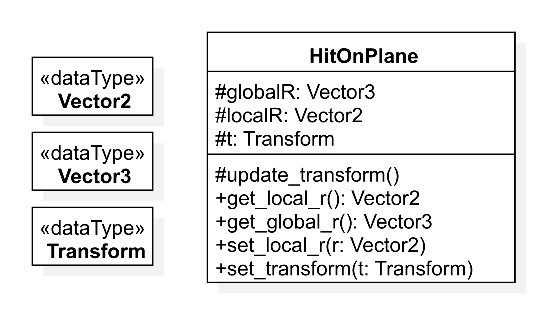
\includegraphics[width=0.45\linewidth]{images/illustrative/complex-hit-class.eps}
    \caption{Класс срабатывания координатного детектора инкапсулирующий координатное преобразование}
    \label{fig:complex-class}
\end{figure}

%В некоторых случаях предметно-ориентированные вычисления сложны, и прибегают к ленивым
%вычислениям, вводя дополнительные флаги контроля, данные кеша и транзитивные хранилища
%для того чтобы снизить потерю производительности на невостребованных элементах состояния.
В ряде случаев предметно-ориентированные вычисления обладают значительной
сложностью и сопровождаются высокой вычислительной нагрузкой. Для повышения
эффективности системы в подобных ситуациях прибегают к ленивым вычислениям,
дополнительно вводя флаги управления, кэш-память и транзитивные хранилища.
Такие меры позволяют минимизировать издержки, связанные с обработкой
невостребованных или редко используемых фрагментов состояния.

%То есть, предметно-ориентированные вычисления требуют реализации механизма согласования
%взаимосвязанных состояний внутри класса координатной метки --- таких, как локальные и
%глобальные координаты в приведённом примере. Возникающая при этом информационная избыточность
%требует введения дополнительных уровней абстракции, инкапсуляции, механизмов
%перенаправления и контроля на уровне события, что оказывает значительное влияние на
%архитектуру последующих программных компонентов обработки. К примеру, при сериализации
%(представление в виде байтовой последовательности для сохранения на диске или ленте)
%и десереализации (восстановлении) описанного в примере объекта принципиально возможно
%появление в программе экземпляра с рассогласованными локальными или глобальными координатами.
Таким образом, предметно-ориентированные вычисления требуют реализации
механизмов согласования взаимозависимых компонентов внутреннего состояния
объекта, как, например, в случае локальных и глобальных координат координатной
метки в трековом детекторе. Возникающая при этом информационная избыточность
предполагает введение дополнительных уровней абстракции и инкапсуляции,
а также реализацию механизмов перенаправления и контроля на уровне
объектной модели события. Эти архитектурные особенности напрямую влияют
на архитектуру и реализацию последующих компонентов программной обработки.

В частности, при \glsprepositional{serialization} (то есть представлении объекта в виде
последовательности байтов для долговременного хранения на внешних носителях)
и последующей \glsprepositional{deserialization} возможно восстановление экземпляра объекта
в рассогласованном состоянии, например, при несовпадении локальных и
глобальных координат вследствие пропуска шагов вычисления или инициализации.

%К аналогичным операциям относятся и другие преобразования на предметно-специфичном уровне
%ответственности, вызванные внешней логикой обработки, включая применение калибровок,
%масштабных преобразований, Фурье-преобразований и т.п.
Аналогичная проблематика возникает и при выполнении других
предметно-специфичных преобразований, инициированных внешними процедурами
обработки, включая применение калибровок, масштабных преобразований,
а также, например, преобразования Фурье и прочие формы предобработки и
согласования представлений.

%Таким образом, (вторым) принципиальным решением при проектировании объектной модели является вопрос,
%насколько \emph{допустима избыточность данных внутри самой модели и как должно быть
%реализовано согласование зависимых элементов}.
В этой связи, одним из принципиальных вопросов при проектировании объектной
модели является определение \emph{допустимого уровня избыточности данных}
внутри структуры события и согласованной с ним \emph{стратегии
согласования зависимых элементов состояния}. Примером наименее избыточных
структур данных могут быть старшие нормальные формы реляционной модели.

%Следует заметить, что архитектура претендующая на высокий уровень общности, не зависящий от конкретного
%эксперимента, не может включать в модель события предметно-ориентированные вычисления ввиду
%многочисленности и противоречивости сценариев использования, а вместо этого должна предоставить
%инфраструктуру в которой определение таких элементов поведения реализуется наиболее упрощено.
Следует подчеркнуть, что архитектура, претендующая на высокий уровень
универсальности и независимости от предметной специфики эксперимента, не может
включать в поведенческое ядро модели события реализацию предметно-ориентированных
вычислений ввиду многочисленности и противоречивости сценариев использования.
Вместо этого она должна предоставлять инфраструктуру, обеспечивающую
максимально простое и декларативное задание соответствующего поведения
в рамках внешней логики прикладного уровня.

Реализацию такого подхода целесообразно осуществить при помощи техник
\glsgenitive{metaprogramming}, опирающихся на интроспективную информацию
о модели события для генерации интерфейсов \acrshort{api}, которые затем
реализуются пользовательскими алгоритмами предметно-ориентированных
вычислений.

Такой подход органично согласуется с предложенной ранее гибридной
методологией разработки ПО, отвечая второму и третьему этапам, в рамках
которых для взаимодействующих алгоритмов фиксируются структурные и
поведенческие аспекты системы.

%В заключении раздела следует заметить, что приведённые рассуждения
%в ограниченной мере справедливы и для т.н. безтриггерных экспериментов.
%В таких экспериментальных установках данные, как правило, обладают той
%или иной степенью гранулярности, обусловленной обычно техническими
%ограничениями. Часто, роль <<события на триггере>> играют временные
%окна (кадры) от потоковых источников данных, которые тем или иным образом
%соотносятся на различных уровнях предобработки (включая циклическую
%буферизацию, различные техники отбора, отыскания корелляций и т.д.),
%прежде чем попасть в персистентные хранилища. Помимо того, что в таких
%системах алгоритмическая насыщенность построения модели события может
%потребовать большей осторожности, чем процедуры реконструкция события,
%попытка построить обобщённую архитектуру предусматривающую работу с данными
%безтриггерного эксперимента обязательно потребует включение в рассмотрение
%систем отбора реализованных на вычислительных платформах различных уровней,
%что существенно увеличит набор вариантов использования системы и её сложность.
В завершение раздела следует отметить, что изложенные выше рассуждения в
определённой степени применимы и к так называемым бестриггерным
экспериментам. В подобных установках исходные данные, как правило,
обладают определённой степенью гранулярности, обусловленной
техническими ограничениями детекторов и средств сбора
информации. Нередко роль событий, зафиксированных триггером
выполняют временные окна (кадры), формируемые потоковыми источниками
данных и соотносимые между собой на различных этапах предварительной
обработки. Эти этапы могут включать циклическую буферизацию,
процедуры быстрого отбора (например, вейвлет-преобразования, поиск по
КД-деревьям), алгоритмы выявления корреляций и другие методы
обработки, предшествующие записи данных в персистентные хранилища.

В контексте данной работы важно, что в таких системах построение
модели события часто сопряжено с более высокой алгоритмической сложностью,
чем в традиционных процедурах реконструкции. Разработка универсальной
архитектуры, способной обрабатывать данные бестриггерных
экспериментов, требует учёта особенностей систем отбора
данных, реализуемых на различных уровнях вычислительной инфраструктуры.
%Это, в свою очередь, существенно расширяет пространство вариантов
%использования программного комплекса и повышает общую сложность
%проектируемой системы.
